\section{Input Sampling}
\label{app:input-sampling}

Observations are typically sampled every five simulator steps.
The actions executed between consecutive observations are included in the interaction history.

\section{Trajectory Construction and Pairing}
\label{app:trajectory-pairing}

\paragraph{Continuous trajectories.}
Each sample follows a continuous simulator trajectory from its history through its future, without intermediate resets or state overrides.
Identical current observations may still conceal differences in velocity or contact state, so we perform task-specific checks of physical-state matching at the start of prediction.
For action delay, we retain the actual queue of pending actions.

\paragraph{Starting positions.}
For tasks in which the two dynamics conditions cannot naturally share a starting position, we exchange their starting positions during generation and verify that the two conditions have identical sets of starting images.
This check reduces the possibility that the starting image alone reveals the condition.

\paragraph{Predictions without history.}
Consider a complete, balanced pair with distinguishable encoded targets.
A deterministic model that ignores history receives the same current observation and future action sequence for both samples and therefore produces the same prediction.
This prediction cannot be strictly closer to each sample's own target than to the other target.
Consequently, such a model scores at most 50\% on the paired future-selection metric in Eq.~\ref{eq:future-score}; ties count as failures.

\section{Action Delay Response Groups}
\label{app:delay-groups}

The delay data retain all 11 delays from 0 to 10 simulator steps.
At the five-step horizon used for the main one-step score, delays of 5--10 produce the same stationary response and are grouped together.
This score therefore uses six distinguishable response groups: 0, 1, 2, 3, 4, and 5--10.

\section{Dataset Statistics and Splits}
\label{app:dataset-splits}

\subsection{Dataset Sizes}

Table~\ref{tab:dataset-sizes} lists the task data used in the training and evaluation comparisons.
Development supports method and checkpoint selection; Test is reserved for final evaluation.
Training sizes exclude the original-environment data used for mixed training.
A pair contains two trajectories with different dynamics conditions; a trajectory count refers to recorded episodes, not to the number of training windows sampled from them.
An evaluation case fixes the current observation and future action sequence and can include histories and targets from several dynamics conditions.

\begin{table*}[!t]
\centering
\small
\caption{Dataset sizes and condition coverage.}
\label{tab:dataset-sizes}
\begin{tabularx}{\textwidth}{@{}lXXX@{}}
\toprule
Task & Training & Development & Test \\
\midrule
Speed & 16,384 trajectories; 32 speeds & 300 cases per speed & 300 cases per speed \\
Pusher displacement & 32,768 pairs & 256 pairs & 256 pairs \\
Arm mass & 32,768 pairs & 256 pairs & 256 pairs \\
Action delay & 56,320 trajectories; 11 delays & 300 cases $\times$ 11 delays & 300 cases $\times$ 11 delays \\
Contact friction & 32,768 pairs & 256 pairs & 256 pairs \\
Motion damping & 32,768 pairs & 256 pairs & 256 pairs \\
Gripper carry rule & 10,000 pairs & 256 pairs & 256 pairs \\
Door traversability & 15,360 trajectories; 96 door positions & 300 cases; 16 door positions & 300 cases; 42 door positions \\
Portal exit & 32,768 pairs & 256 pairs & 256 pairs \\
\bottomrule
\end{tabularx}
\end{table*}

The action delay counts refer to the dataset covering all delays from 0 to 10 simulator steps.
Its Training split contains 5,120 base cases, each simulated under all 11 delays, giving 56,320 trajectories.
Development and Test each contain 300 base cases, again evaluated under all 11 delays.
Door Training contains 7,680 trajectories for each of the passable and blocked rules.

Several examples can share a source episode: pusher displacement can use multiple action windows from one episode, and forward and mirrored damping examples can share a source.
The 10,000 gripper carry training pairs use 10,000 distinct source episodes.

\subsection{Paired Dynamics Conditions}

Pusher displacement uses action gains of 60 and 140.
Contact friction uses coefficients 0.05 and 0.80 between the pusher and the object.
Motion damping fixes effective contact friction at 0.25 and uses simulator damping settings 0.2 and 1.0; here 0.2 gives faster decay, while 1.0 applies no additional decay.
Arm mass uses densities of 500 and 1,500 for the MuJoCo arm link and finger geometry; the hand link retains its original density.
Gripper carry changes whether the closed gripper carries the cube.
Portal exit uses two exit rules for the same entrance, with paired trajectories reaching the shared query state before entering it.
The numeric settings are simulator parameters, not additional model inputs.

\subsection{Speed Values and Door Positions}

Table~\ref{tab:speed-values} lists the speed values used for Training and evaluation.
Development and Test use the same evaluation speeds but different interaction trajectories.
Each split contains 300 cases for each of the 14 evaluated speeds, or 4,200 cases in total before comparing histories from different speeds.
The main task results use the unseen speeds within the training range.

\begin{table}[!ht]
\centering
\small
\caption{Speed values in the benchmark. The four evaluation groups are used in both Development and Test. Interpolation values lie within the Training range but are absent from Training.}
\label{tab:speed-values}
\begin{tabularx}{\linewidth}{@{}lX@{}}
\toprule
Setting & Speed values \\
\midrule
Training & 2.6, 2.7, 2.8, 2.9, 3.1, 3.3, 3.5, 3.7, 3.8, 3.9, 4.1, 4.2, 4.4, 4.5, 4.7, 5.0, 5.1, 5.3, 5.5, 5.7, 5.9, 6.1, 6.2, 6.3, 6.6, 6.7, 6.8, 7.0, 7.2, 7.3, 7.8, 7.9 \\
\midrule
Seen speeds & 3.1, 5.1, 7.0 \\
Interpolation & 3.4, 4.8, 6.9 \\
Lower extrapolation & 1.75, 1.95, 2.15, 2.35 \\
Upper extrapolation & 8.25, 8.75, 9.5, 10.25 \\
\bottomrule
\end{tabularx}
\end{table}

Door position is specified by an integer coordinate along the wall.
Test uses the 42 positions $30+4k$, where $k=0,\ldots,41$.
Development uses the 16 positions 65, 77, 79, 87, 112, 115, 131, 152, 167, 169, 171, 172, 175, 180, 183, 185.
Training uses the integers from 36 through 188 after excluding all Development and Test positions and the additional unused positions 40, 127, and 132, leaving 96 positions.
The three position sets are disjoint.
Both passable and blocked rules are used across the splits; the test distinction is the door position, not a new rule.

\subsection{Split Checks and Model Inputs}

Split checks use source episode identifiers, trajectory template identifiers, or observation hashes, as appropriate for each task.
Speed Development uses independently generated initial configurations and excludes initial states and current observations that duplicate Test cases.
For Door, we also check the position sets listed above for overlap.

Hidden dynamics values, simulator states, and pair identifiers are retained for data generation, validation, and scoring.
They are not passed to the prediction model, which receives only the visual observations and actions defined in Sec.~\ref{sec:problem}.


\section{Evaluation Details}
\label{app:evaluation-details}

\paragraph{Paired tasks.}
The strict comparisons in Eq.~\ref{eq:future-score} do not count ties as correct.
The two comparisons within a pair are dependent.
Appendix~\ref{app:trajectory-pairing} explains the upper bound for a deterministic model that ignores history.

\paragraph{Speed.}
For each target speed, accuracy is the proportion of cases in which matching history gives strictly lower prediction error than every alternative history.
We then average accuracy equally across target speeds.
Ties do not count as correct: if all histories produce the same prediction, accuracy is zero.
The main results use the interpolation speeds listed in Appendix~\ref{app:dataset-splits}.

\paragraph{Action delay.}
We select the candidate true future with the lowest mean squared error, resolving ties in favor of the smaller delay.
The prediction is correct when the selected delay and the true delay belong to the same response group.
Within each case, we first average correctness over delays in each group, then average equally across the six groups defined in Appendix~\ref{app:delay-groups}.
The final accuracy is the mean over cases.

\paragraph{Door traversability.}
For a prediction made with matching history, we compare the mean squared errors to the passage and blockage futures.
The prediction is correct only if the error to the true future is strictly smaller than the error to the alternative future.
Accuracy is averaged over cases and the two rules; ties do not count as correct.

\paragraph{Multi-step prediction horizons.}
Each prediction step advances five simulator steps.
We measure prediction errors at 5, 10, 15, 20, and 25 simulator steps after the current observation.

\paragraph{Within-scene aggregation.}
Let $z_{qkct}$ and $\hat z_{qkct}$ denote the true and predicted future representations for scene $q$, dynamics condition $k$, action sequence $c$, and prediction time $t$.
With $K_q$ conditions, $C_q$ shared action sequences, and $T=5$ prediction times, the errors used in Eq.~\ref{eq:complete-error} are
\[
\begin{aligned}
L_q&=\frac{1}{K_qC_qT}\sum_{k,c,t}\|\hat z_{qkct}-z_{qkct}\|^2,\\
B_q&=\frac{1}{K_qC_qT}\sum_{k,c,t}\|z_{qkct}-\bar z_{qct}\|^2,\\
\bar z_{qct}&=\frac{1}{K_q}\sum_k z_{qkct}.
\end{aligned}
\]
L2World tests history dependence by shuffling context observations~\cite{wang2026context}; our controls instead swap histories between dynamics conditions.
For history controls, $E_+$ and $E_-$ sum the matching- and mismatched-history scene errors using the same averaging over conditions, action sequences, and prediction times.
When a sample has multiple mismatched histories, their errors are averaged equally.
A positive $G_H$ indicates that matching history reduces error; it does not imply a low complete prediction error.

\paragraph{Mean-future reference.}
The reference in Eq.~\ref{eq:complete-error} is used only for scoring and is never provided to the model.
The ratio is defined only when $\sum_q B_q>0$.
When conditions share the current observation and future actions and are equally weighted, a deterministic model that ignores history cannot achieve $E/B<1$: it must make the same prediction across conditions, and the mean-future reference minimizes the error of such a prediction.

\paragraph{Response error settings.}
We specify the prediction horizon for each NRE analysis.
The ratio in Eq.~\ref{eq:response-error} is defined only when $\sum_i\|\Delta z_i\|^2>0$.
NRE equal to 1 does not by itself show that a model ignores history.
Errors shared by both predictions cancel in the difference, so an exact conditional response does not imply exact complete predictions.

\paragraph{Uncertainty estimates.}
\label{app:result-uncertainty}
For multi-step errors, we use cluster bootstrap resampling~\cite{efron1993bootstrap,field2007cluster} at the level of source trajectories or scenes, retaining related samples together.
These intervals describe scene-sampling uncertainty for the evaluated checkpoints, not variability across training runs.

\paragraph{Interpreting multiple metrics.}
The metrics describe different aspects of the same predictions and are not independent pieces of evidence.

\clearpage
\onecolumn
\section{Scoring Controls}
\label{app:scoring-controls}

We validate the paired scorer using constructed predictions on 256 Test pusher-displacement scenes, separately in the target representations of LeWM Original and Original $\rightarrow$ Mixed (Frozen Encoder).
The queries use a nonzero action candidate and the five-step prediction horizon; the predictor is not run for this check.
Both representations give the results below.
With $m=(z_A+z_B)/2$, even predictions $m+0.001(z_k-m)$ select the correct future while recovering only a tiny fraction of the true response.
This control explains why we report response error alongside task accuracy.
It verifies the scorer on these queries, not physical calibration across all representations.

\begin{center}\small
\begin{tabular}{@{}lrrr@{}}
\toprule
Constructed prediction & Accuracy (\%) & \shortstack{History\\win rate (\%)} & NRE\\
\midrule
True target for each condition & 100 & 100 & 0\\
Same target $z_A$ for both conditions & 50 & 0 & 1\\
Same midpoint $m$ for both conditions & 0 & 0 & 1\\
Swapped true targets & 0 & 0 & 4\\
$m+0.001(z_k-m)$ for condition $k$ & 100 & 100 & 0.998001\\
\bottomrule\end{tabular}\end{center}

\section{Training and Diagnostic Settings}
\label{app:training-settings}

\paragraph{Optimization.}
The training recipe specifies 10 epochs per stage on eight GPUs, with 128 windows per device and no gradient accumulation, giving a global batch size of 1,024.
LeWM and PLDM use AdamW with learning rate $5\times10^{-5}$ and weight decay 0.001.
DINO-WM uses learning rate $5\times10^{-4}$ and zero weight decay; its pretrained DINOv2-small visual encoder remains frozen.
The models retain their respective prediction and regularization losses.
The Original $\rightarrow$ Mixed schemes load model weights but reset optimizer state.
Encoder freezing fixes both parameters and training-state buffers; it does not freeze the projector or action encoder.

\paragraph{Input and sampling.}
The standard setup uses three observation frames, five simulator steps between frames, and a one-frame prediction target.
Action delay mixed training instead uses seven-frame history.
The original-environment data are the TwoRoom, PushT, Reacher, and Cube datasets released with LeWM; each task uses only the dataset for its environment.
Only the ContextWorld Training split is mixed into training.
For component lengths $N_{\mathrm{orig}}$ and $N_{\mathrm{CW}}$, the mixture has a nominal epoch length of $2\max(N_{\mathrm{orig}},N_{\mathrm{CW}})$ windows before partitioning and batching, with equal counts from the two components.
The smaller component is sampled repeatedly.
Consequently, equal epoch counts do not guarantee equal update counts across data scales, and the two-stage schemes include additional original-environment training.

\paragraph{Prediction diagnostics.}
The main task comparison uses Test.
The multi-step and history diagnostics below use Test and the same checkpoints as the main task comparison.
Multi-step evaluation covers 2,436 source scenes across all nine tasks and predicts at 5, 10, 15, 20, and 25 simulator steps using only the initial observed history.
The candidate actions and multi-step targets extend the one-step task queries.
For gripper carry, we replay all 256 held-out source cases and render their histories and extended futures together, preserving the paired current-observation constraint without mixing stored images with newly rendered futures. These coherent replays retain the source conditions and actions but do not reproduce the stored images exactly; the original task-query evaluation is unchanged.
Figure~\ref{fig:multistep-prediction} reports $E_t/B_t$: prediction and mean-future errors are summed over queries separately at each horizon, normalized within each checkpoint, then averaged equally over training repetitions. The aggregate $E/B$ instead combines errors over all horizons before division; it is not the arithmetic mean of these per-horizon ratios.
Each checkpoint is scored separately, and matching training repetitions are then averaged equally.
Intervals use 4,000 source-cluster bootstrap samples; all conditions, actions, and times from a source remain together.
They condition on the evaluated checkpoints and do not estimate variation from retraining the model.
Original action-delay checkpoints do not have the native seven-frame interface and are excluded from this comparison.
DINO-WM has no jointly updated visual-encoder scheme; its comparable Original $\rightarrow$ Mixed results cover Speed, damping, and gripper carry.

\paragraph{Planning evaluation.}
CEM results measure success in the original environments, with no hidden-dynamics history intervention.
Most checkpoint evaluations use six evaluation seeds with 50 episodes each; some original LeWM and PLDM references use three sets of 100 episodes or an aggregated 300-episode result.
Evaluation repetitions are pooled within each checkpoint, then training repetitions are averaged equally.
A single original-environment checkpoint supplies the reference for all tasks from that environment; these repeated entries are not independent experiments.

\paragraph{Training-query analysis.}
The friction and damping comparisons use 32,768 training pairs, identical original-environment initialization within each task, and the same 50/50 mixture, batch size, and duration.
We evaluate 512 fixed training pairs and 256 Test pairs per task at epochs 5 and 10, predicting the next observation five simulator steps ahead.
Loss summaries use the logged mixed-training batches, approximately 50--70 records per epoch, rather than every training batch.
Checkpoints and logs are aligned by update step.
The curves show recorded means and batch interquartile ranges; loss medians give the same monotonic direction for friction joint training from epochs 5 to 10.
NRE is evaluated in each checkpoint's target representation and is not a common physical error across checkpoints.
For damping with the encoder frozen, prediction loss changes by only $-0.39\%$ between these endpoints and fluctuates in between. The late-training plateau is consistent with the loss approaching convergence.

\begin{figure}[htbp]
\centering
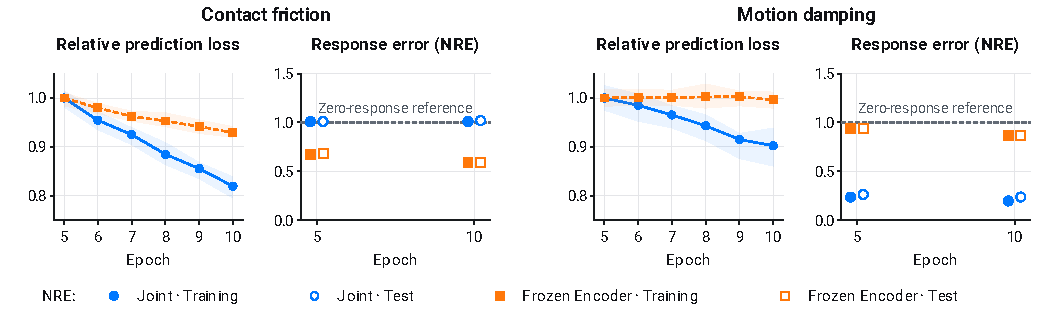
\includegraphics[width=\textwidth]{figures/training_evidence_full.pdf}
\caption{\textbf{Training loss and conditional responses across tasks and schemes.} Within each task, PLDM Joint and Frozen Encoder share Original initialization. Loss is normalized to epoch 5; shading shows batch interquartile ranges. Blue denotes prediction loss and orange denotes NRE; circles denote Joint and squares denote Frozen Encoder. NRE uses filled markers for Training and open markers for Test, evaluated only at epochs 5 and 10. Small horizontal offsets separate the two splits; 1 marks the zero-response reference. Loss uses mixed batches, whereas NRE uses fixed paired task queries.}
\label{fig:training-evidence-full}
\end{figure}

\section{Additional Results}
\label{app:additional-results}

Table~\ref{tab:test-metrics-full} reports all three Test adaptation metrics with training-run counts and standard deviations.
Table~\ref{tab:test-diagnostics} combines Test history and response metrics with multi-step prediction errors and original-environment planning results.
History win rate measures strict error reduction from matching history on the task queries; NRE measures the conditional response on those queries.
$E/B$ uses the extended multi-step action panels and includes errors shared by both conditions.
Because the query sets and prediction horizons differ, these columns should not be treated as measurements of the same event.
All latent errors are computed in the checkpoint's own target representation.

% BEGIN GENERATED PAPER RESULTS
% Generated by paper/generate_test_tables.py; do not edit values.
\begingroup
\small
\setlength{\tabcolsep}{3pt}
\renewcommand{\arraystretch}{1.08}
\begin{longtable}{@{}>{\raggedright\arraybackslash}p{2.55cm}l>{\raggedright\arraybackslash}p{4.05cm}rrrr@{}}
\caption{\textbf{Complete Test adaptation metrics.} Each row uses the same evaluated checkpoints for all three metrics. Entries are means $\pm$ sample standard deviations across $n$ training runs; a single run has no sample standard deviation. Accuracy and History are percentages; NRE is dimensionless. Speed uses unseen interpolation speeds, and its Accuracy and History use the same scoring rule. Action delay uses seven-frame history. Only available comparable configurations are listed.}\label{tab:test-metrics-full}\label{tab:test-variability}\\
\toprule
Task & Model & Training scheme & $n$ & Accuracy $\uparrow$ & History $\uparrow$ & NRE $\downarrow$ \\
\midrule\endfirsthead
\toprule
Task & Model & Training scheme & $n$ & Accuracy $\uparrow$ & History $\uparrow$ & NRE $\downarrow$ \\
\midrule\endhead
\bottomrule\endfoot
Speed & LeWM & Original & 3 & $58.04\pm1.70$ & $58.04\pm1.70$ & $0.896\pm0.027$ \\
Speed & LeWM & Mixed & 3 & $98.19\pm0.57$ & $98.19\pm0.57$ & $0.042\pm0.011$ \\
Speed & LeWM & Original $\to$ Mixed (Joint) & 1 & 96.89 & 96.89 & 0.055 \\
Speed & LeWM & Original $\to$ Mixed\newline (Frozen Encoder) & 1 & 98.44 & 98.44 & 0.030 \\
Speed & PLDM & Original & 3 & $48.41\pm4.33$ & $48.41\pm4.33$ & $0.922\pm0.026$ \\
Speed & PLDM & Mixed & 3 & $96.78\pm2.02$ & $96.78\pm2.02$ & $0.084\pm0.013$ \\
Speed & PLDM & Original $\to$ Mixed (Joint) & 1 & 98.33 & 98.33 & 0.047 \\
Speed & PLDM & Original $\to$ Mixed\newline (Frozen Encoder) & 1 & 96.44 & 96.44 & 0.062 \\
Speed & DINO-WM & Original & 1 & 57.11 & 57.11 & 0.919 \\
Speed & DINO-WM & Mixed & 3 & $59.41\pm3.87$ & $59.41\pm3.87$ & $0.961\pm0.011$ \\
Speed & DINO-WM & Original $\to$ Mixed & 1 & 84.78 & 84.78 & 0.411 \\
\addlinespace[3pt]
Pusher displacement & LeWM & Original & 3 & $48.96\pm1.00$ & $28.32\pm12.76$ & $1.018\pm0.016$ \\
Pusher displacement & LeWM & Mixed & 1 & 50.78 & 79.10 & 0.974 \\
Pusher displacement & LeWM & Original $\to$ Mixed (Joint) & 1 & 91.80 & 99.02 & 0.215 \\
Pusher displacement & LeWM & Original $\to$ Mixed\newline (Frozen Encoder) & 1 & 97.46 & 98.83 & 0.128 \\
Pusher displacement & PLDM & Original & 3 & $45.57\pm1.88$ & $9.38\pm4.20$ & $1.058\pm0.012$ \\
Pusher displacement & PLDM & Mixed & 1 & 56.25 & 68.16 & 0.835 \\
Pusher displacement & PLDM & Original $\to$ Mixed (Joint) & 1 & 59.18 & 73.44 & 0.740 \\
Pusher displacement & PLDM & Original $\to$ Mixed\newline (Frozen Encoder) & 1 & 98.63 & 99.80 & 0.101 \\
Pusher displacement & DINO-WM & Original & 1 & 38.48 & 9.38 & 1.127 \\
Pusher displacement & DINO-WM & Mixed & 1 & 97.66 & 99.61 & 0.394 \\
\addlinespace[3pt]
Arm mass & LeWM & Original & 3 & $50.07\pm0.11$ & $51.63\pm0.60$ & $0.977\pm0.002$ \\
Arm mass & LeWM & Mixed & 1 & 85.74 & 89.84 & 0.045 \\
Arm mass & LeWM & Original $\to$ Mixed (Joint) & 1 & 87.30 & 93.36 & 0.038 \\
Arm mass & LeWM & Original $\to$ Mixed\newline (Frozen Encoder) & 1 & 77.15 & 86.52 & 0.346 \\
Arm mass & PLDM & Original & 3 & $51.82\pm1.30$ & $66.99\pm9.68$ & $0.921\pm0.016$ \\
Arm mass & PLDM & Mixed & 1 & 91.02 & 93.55 & 0.031 \\
Arm mass & PLDM & Original $\to$ Mixed (Joint) & 1 & 84.77 & 90.82 & 0.073 \\
Arm mass & PLDM & Original $\to$ Mixed\newline (Frozen Encoder) & 1 & 81.84 & 89.26 & 0.213 \\
Arm mass & DINO-WM & Original & 1 & 50.78 & 61.33 & 0.977 \\
Arm mass & DINO-WM & Mixed & 1 & 78.32 & 88.09 & 0.673 \\
\addlinespace[3pt]
Action delay & LeWM & Mixed & 3 & $97.70\pm0.59$ & $99.18\pm0.38$ & $0.013\pm0.002$ \\
Action delay & PLDM & Mixed & 3 & $100.00\pm0.00$ & $100.00\pm0.00$ & $0.006\pm0.001$ \\
Action delay & DINO-WM & Mixed & 3 & $16.65\pm0.03$ & $19.45\pm0.11$ & $1.000\pm0.000$ \\
\addlinespace[3pt]
Contact friction & LeWM & Original & 3 & $49.93\pm0.23$ & $50.13\pm0.63$ & $1.001\pm0.004$ \\
Contact friction & LeWM & Mixed & 1 & 50.00 & 49.41 & 1.000 \\
Contact friction & LeWM & Original $\to$ Mixed (Joint) & 1 & 50.39 & 54.30 & 0.999 \\
Contact friction & LeWM & Original $\to$ Mixed\newline (Frozen Encoder) & 1 & 86.13 & 92.77 & 0.429 \\
Contact friction & PLDM & Original & 3 & $50.00\pm0.34$ & $49.09\pm1.58$ & $1.014\pm0.010$ \\
Contact friction & PLDM & Mixed & 1 & 50.00 & 48.63 & 1.001 \\
Contact friction & PLDM & Original $\to$ Mixed (Joint) & 1 & 50.00 & 46.48 & 1.020 \\
Contact friction & PLDM & Original $\to$ Mixed\newline (Frozen Encoder) & 1 & 73.63 & 83.59 & 0.595 \\
Contact friction & DINO-WM & Original & 1 & 50.39 & 47.66 & 1.015 \\
Contact friction & DINO-WM & Mixed & 1 & 84.18 & 92.19 & 0.648 \\
\addlinespace[3pt]
Motion damping & LeWM & Original & 3 & $50.00\pm0.00$ & $48.63\pm1.60$ & $1.007\pm0.009$ \\
Motion damping & LeWM & Mixed & 1 & 50.00 & 48.24 & 1.004 \\
Motion damping & LeWM & Original $\to$ Mixed (Joint) & 1 & 50.00 & 49.61 & 1.001 \\
Motion damping & LeWM & Original $\to$ Mixed\newline (Frozen Encoder) & 1 & 53.91 & 61.91 & 0.958 \\
Motion damping & PLDM & Original & 3 & $50.26\pm0.30$ & $50.52\pm0.63$ & $0.947\pm0.007$ \\
Motion damping & PLDM & Mixed & 1 & 58.20 & 55.86 & 2.435 \\
Motion damping & PLDM & Original $\to$ Mixed (Joint) & 1 & 79.88 & 81.84 & 0.237 \\
Motion damping & PLDM & Original $\to$ Mixed\newline (Frozen Encoder) & 1 & 54.49 & 64.26 & 0.867 \\
Motion damping & DINO-WM & Original & 1 & 49.80 & 49.61 & 1.014 \\
Motion damping & DINO-WM & Mixed & 1 & 56.45 & 65.23 & 1.042 \\
Motion damping & DINO-WM & Original $\to$ Mixed & 1 & 55.27 & 61.13 & 1.111 \\
\addlinespace[3pt]
Gripper carry rule & LeWM & Original & 3 & $52.21\pm1.11$ & $73.76\pm1.97$ & $0.909\pm0.029$ \\
Gripper carry rule & LeWM & Mixed & 1 & 50.00 & 49.80 & 1.000 \\
Gripper carry rule & LeWM & Original $\to$ Mixed (Joint) & 1 & 50.00 & 52.34 & 0.997 \\
Gripper carry rule & LeWM & Original $\to$ Mixed\newline (Frozen Encoder) & 1 & 76.37 & 84.57 & 0.271 \\
Gripper carry rule & PLDM & Original & 3 & $50.78\pm0.20$ & $57.42\pm1.35$ & $0.937\pm0.007$ \\
Gripper carry rule & PLDM & Mixed & 1 & 49.80 & 50.78 & 0.997 \\
Gripper carry rule & PLDM & Original $\to$ Mixed (Joint) & 1 & 50.20 & 54.30 & 0.982 \\
Gripper carry rule & PLDM & Original $\to$ Mixed\newline (Frozen Encoder) & 1 & 52.93 & 57.81 & 0.606 \\
Gripper carry rule & DINO-WM & Original & 1 & 50.00 & 50.59 & 1.000 \\
Gripper carry rule & DINO-WM & Mixed & 1 & 60.16 & 77.34 & 0.892 \\
Gripper carry rule & DINO-WM & Original $\to$ Mixed & 1 & 62.89 & 80.27 & 0.871 \\
\addlinespace[3pt]
Door traversability & LeWM & Original & 3 & $50.33\pm0.00$ & $50.94\pm2.84$ & $0.996\pm0.003$ \\
Door traversability & LeWM & Mixed & 3 & $99.83\pm0.29$ & $100.00\pm0.00$ & $0.041\pm0.018$ \\
Door traversability & LeWM & Original $\to$ Mixed (Joint) & 1 & 99.83 & 100.00 & 0.038 \\
Door traversability & LeWM & Original $\to$ Mixed\newline (Frozen Encoder) & 1 & 100.00 & 100.00 & 0.036 \\
Door traversability & PLDM & Original & 3 & $50.06\pm0.10$ & $51.50\pm0.67$ & $0.997\pm0.002$ \\
Door traversability & PLDM & Mixed & 3 & $100.00\pm0.00$ & $100.00\pm0.00$ & $0.022\pm0.005$ \\
Door traversability & PLDM & Original $\to$ Mixed (Joint) & 1 & 100.00 & 100.00 & 0.023 \\
Door traversability & PLDM & Original $\to$ Mixed\newline (Frozen Encoder) & 1 & 100.00 & 100.00 & 0.048 \\
Door traversability & DINO-WM & Original & 1 & 50.00 & 64.33 & 0.985 \\
Door traversability & DINO-WM & Mixed & 3 & $100.00\pm0.00$ & $100.00\pm0.00$ & $0.217\pm0.003$ \\
\addlinespace[3pt]
Portal exit & LeWM & Original & 3 & $50.07\pm0.11$ & $51.95\pm0.70$ & $0.990\pm0.003$ \\
Portal exit & LeWM & Mixed & 1 & 50.78 & 76.37 & 0.922 \\
Portal exit & LeWM & Original $\to$ Mixed (Joint) & 1 & 50.39 & 66.80 & 0.934 \\
Portal exit & LeWM & Original $\to$ Mixed\newline (Frozen Encoder) & 1 & 77.93 & 94.34 & 0.264 \\
Portal exit & PLDM & Original & 3 & $50.07\pm0.11$ & $51.50\pm0.30$ & $0.996\pm0.001$ \\
Portal exit & PLDM & Mixed & 1 & 72.27 & 79.10 & 0.128 \\
Portal exit & PLDM & Original $\to$ Mixed (Joint) & 1 & 52.54 & 61.52 & 0.708 \\
Portal exit & PLDM & Original $\to$ Mixed\newline (Frozen Encoder) & 1 & 91.21 & 98.83 & 0.191 \\
Portal exit & DINO-WM & Original & 1 & 50.78 & 56.45 & 0.996 \\
Portal exit & DINO-WM & Mixed & 1 & 100.00 & 100.00 & 0.142 \\
\addlinespace[3pt]
\end{longtable}\endgroup

\begingroup
\small
\setlength{\tabcolsep}{3pt}
\renewcommand{\arraystretch}{1.15}
\begin{longtable}{@{}p{1.8cm}lp{3.65cm}rrrp{2.5cm}r@{}}
\caption{Test prediction diagnostics and original-environment CEM. Entries average the available training repetitions; $E/B$ intervals are 95\% source-bootstrap intervals. History win rate and CEM are percentages. Scheme names match the main text.}\label{tab:test-diagnostics}\\
\toprule
Task & Model & Scheme & \shortstack{History\\win rate $\uparrow$} & NRE $\downarrow$ & $E/B$ $\downarrow$ & $E/B$ interval & CEM $\uparrow$\\
\midrule
\endfirsthead
\toprule
Task & Model & Scheme & \shortstack{History\\win rate $\uparrow$} & NRE $\downarrow$ & $E/B$ $\downarrow$ & $E/B$ interval & CEM $\uparrow$\\
\midrule
\endhead
\bottomrule
\endfoot
Speed & LeWM & Original & 58.04 & 0.896 & 1.512 & [1.491, 1.533] & 92.44 \\
Speed & LeWM & Mixed & 98.19 & 0.042 & 0.368 & [0.350, 0.388] & 97.44 \\
Speed & LeWM & Original $\rightarrow$ Mixed (Joint) & 96.89 & 0.055 & 0.399 & [0.376, 0.423] & 97.00 \\
Speed & LeWM & Original $\rightarrow$ Mixed (Frozen Encoder) & 98.44 & 0.030 & 0.145 & [0.133, 0.157] & 95.00 \\
Speed & PLDM & Original & 48.41 & 0.922 & 3.446 & [3.366, 3.542] & 90.56 \\
Speed & PLDM & Mixed & 96.78 & 0.084 & 0.515 & [0.492, 0.539] & 96.89 \\
Speed & PLDM & Original $\rightarrow$ Mixed (Joint) & 98.33 & 0.047 & 0.380 & [0.355, 0.408] & 96.33 \\
Speed & PLDM & Original $\rightarrow$ Mixed (Frozen Encoder) & 96.44 & 0.062 & 0.308 & [0.290, 0.326] & 98.00 \\
Speed & DINO-WM & Original & 57.11 & 0.919 & 1.967 & [1.949, 1.987] & 100.00 \\
Speed & DINO-WM & Mixed & 59.41 & 0.961 & 2.086 & [2.054, 2.123] & 99.89 \\
Speed & DINO-WM & Original $\rightarrow$ Mixed & 84.78 & 0.411 & 0.886 & [0.851, 0.924] & 100.00 \\
\midrule
Pusher displacement & LeWM & Original & 28.32 & 1.018 & 2.279 & [2.211, 2.354] & 82.22 \\
Pusher displacement & LeWM & Mixed & 79.10 & 0.974 & 3.779 & [3.596, 3.968] & 78.67 \\
Pusher displacement & LeWM & Original $\rightarrow$ Mixed (Joint) & 99.02 & 0.215 & 2.426 & [2.353, 2.504] & 86.00 \\
Pusher displacement & LeWM & Original $\rightarrow$ Mixed (Frozen Encoder) & 98.83 & 0.128 & 1.436 & [1.365, 1.510] & 73.67 \\
Pusher displacement & PLDM & Original & 9.38 & 1.058 & 2.386 & [2.332, 2.442] & 75.67 \\
Pusher displacement & PLDM & Mixed & 68.16 & 0.835 & 6.284 & [6.001, 6.589] & 61.33 \\
Pusher displacement & PLDM & Original $\rightarrow$ Mixed (Joint) & 73.44 & 0.740 & 3.720 & [3.604, 3.840] & 72.00 \\
Pusher displacement & PLDM & Original $\rightarrow$ Mixed (Frozen Encoder) & 99.80 & 0.101 & 1.448 & [1.397, 1.501] & 59.33 \\
Pusher displacement & DINO-WM & Original & 9.38 & 1.127 & 3.140 & [3.024, 3.261] & 76.67 \\
Pusher displacement & DINO-WM & Mixed & 99.61 & 0.394 & 1.931 & [1.884, 1.981] & 76.67 \\
\midrule
Arm mass & LeWM & Original & 51.63 & 0.977 & 741.737 & [644.066, 844.093] & 55.89 \\
Arm mass & LeWM & Mixed & 89.84 & 0.045 & 51.802 & [47.895, 56.217] & 58.00 \\
Arm mass & LeWM & Original $\rightarrow$ Mixed (Joint) & 93.36 & 0.038 & 47.590 & [44.059, 51.609] & 59.00 \\
Arm mass & LeWM & Original $\rightarrow$ Mixed (Frozen Encoder) & 86.52 & 0.346 & 33.070 & [30.472, 35.587] & 59.67 \\
Arm mass & PLDM & Original & 66.99 & 0.921 & 19.698 & [17.799, 21.952] & 69.67 \\
Arm mass & PLDM & Mixed & 93.55 & 0.031 & 13.815 & [12.861, 14.967] & 51.67 \\
Arm mass & PLDM & Original $\rightarrow$ Mixed (Joint) & 90.82 & 0.073 & 46.000 & [42.230, 50.596] & 58.67 \\
Arm mass & PLDM & Original $\rightarrow$ Mixed (Frozen Encoder) & 89.26 & 0.213 & 17.048 & [16.034, 18.176] & 89.00 \\
Arm mass & DINO-WM & Original & 61.33 & 0.977 & 49.483 & [46.626, 52.747] & 90.67 \\
Arm mass & DINO-WM & Mixed & 88.09 & 0.673 & 14.166 & [13.764, 14.537] & 75.00 \\
\midrule
Action delay & LeWM & Mixed & 99.18 & 0.013 & 1.429 & [1.406, 1.453] & 87.33 \\
Action delay & PLDM & Mixed & 100.00 & 0.006 & 1.818 & [1.804, 1.832] & 90.89 \\
Action delay & DINO-WM & Mixed & 19.45 & 1.000 & 66.094 & [65.265, 66.948] & 33.56 \\
\midrule
Contact friction & LeWM & Original & 50.13 & 1.001 & 2.716 & [2.642, 2.791] & 82.22 \\
Contact friction & LeWM & Mixed & 49.41 & 1.000 & 2.727 & [2.678, 2.781] & 76.67 \\
Contact friction & LeWM & Original $\rightarrow$ Mixed (Joint) & 54.30 & 0.999 & 2.717 & [2.677, 2.757] & 86.00 \\
Contact friction & LeWM & Original $\rightarrow$ Mixed (Frozen Encoder) & 92.77 & 0.429 & 2.902 & [2.843, 2.960] & 83.33 \\
Contact friction & PLDM & Original & 49.09 & 1.014 & 3.809 & [3.686, 3.940] & 75.67 \\
Contact friction & PLDM & Mixed & 48.63 & 1.001 & 6.392 & [6.077, 6.741] & 65.67 \\
Contact friction & PLDM & Original $\rightarrow$ Mixed (Joint) & 46.48 & 1.020 & 7.236 & [6.961, 7.541] & 73.33 \\
Contact friction & PLDM & Original $\rightarrow$ Mixed (Frozen Encoder) & 83.59 & 0.595 & 4.536 & [4.408, 4.666] & 79.67 \\
Contact friction & DINO-WM & Original & 47.66 & 1.015 & 6.252 & [5.971, 6.531] & 76.67 \\
Contact friction & DINO-WM & Mixed & 92.19 & 0.648 & 3.695 & [3.611, 3.776] & 75.67 \\
\midrule
Motion damping & LeWM & Original & 48.63 & 1.007 & 5.341 & [5.105, 5.611] & 82.22 \\
Motion damping & LeWM & Mixed & 48.24 & 1.004 & 248.446 & [216.917, 288.116] & 78.00 \\
Motion damping & LeWM & Original $\rightarrow$ Mixed (Joint) & 49.61 & 1.001 & 87.139 & [77.847, 98.646] & 88.33 \\
Motion damping & LeWM & Original $\rightarrow$ Mixed (Frozen Encoder) & 61.91 & 0.958 & 8.316 & [7.878, 8.794] & 84.33 \\
Motion damping & PLDM & Original & 50.52 & 0.947 & 6.216 & [5.937, 6.535] & 75.67 \\
Motion damping & PLDM & Mixed & 55.86 & 2.435 & 21.427 & [18.508, 25.342] & 61.00 \\
Motion damping & PLDM & Original $\rightarrow$ Mixed (Joint) & 81.84 & 0.237 & 8.323 & [8.060, 8.597] & 70.00 \\
Motion damping & PLDM & Original $\rightarrow$ Mixed (Frozen Encoder) & 64.26 & 0.867 & 5.680 & [5.431, 5.959] & 78.33 \\
Motion damping & DINO-WM & Original & 49.61 & 1.014 & 8.442 & [8.184, 8.713] & 76.67 \\
Motion damping & DINO-WM & Mixed & 65.23 & 1.042 & 7.292 & [7.117, 7.484] & 76.67 \\
Motion damping & DINO-WM & Original $\rightarrow$ Mixed & 61.13 & 1.111 & 6.975 & [6.800, 7.165] & 76.00 \\
\midrule
Gripper carry rule & LeWM & Original & 73.76 & 0.909 & 10.647 & [9.807, 11.634] & 65.44 \\
Gripper carry rule & LeWM & Mixed & 49.80 & 1.000 & 170.794 & [132.250, 222.804] & 61.33 \\
Gripper carry rule & LeWM & Original $\rightarrow$ Mixed (Joint) & 52.34 & 0.997 & 12.148 & [10.850, 13.816] & 71.00 \\
Gripper carry rule & LeWM & Original $\rightarrow$ Mixed (Frozen Encoder) & 84.57 & 0.271 & 11.149 & [10.363, 12.008] & 67.00 \\
Gripper carry rule & PLDM & Original & 57.42 & 0.937 & 11.994 & [9.809, 15.328] & 53.44 \\
Gripper carry rule & PLDM & Mixed & 50.78 & 0.997 & 138.687 & [115.564, 166.941] & 55.00 \\
Gripper carry rule & PLDM & Original $\rightarrow$ Mixed (Joint) & 54.30 & 0.982 & 26.192 & [23.629, 29.169] & 56.67 \\
Gripper carry rule & PLDM & Original $\rightarrow$ Mixed (Frozen Encoder) & 57.81 & 0.606 & 25.681 & [20.138, 33.793] & 56.67 \\
Gripper carry rule & DINO-WM & Original & 50.59 & 1.000 & 40.837 & [39.662, 42.051] & 72.67 \\
Gripper carry rule & DINO-WM & Mixed & 77.34 & 0.892 & 11.402 & [11.088, 11.709] & 71.67 \\
Gripper carry rule & DINO-WM & Original $\rightarrow$ Mixed & 80.27 & 0.871 & 11.286 & [10.982, 11.585] & 73.67 \\
\midrule
Door traversability & LeWM & Original & 50.94 & 0.996 & 5.255 & [5.151, 5.364] & 92.44 \\
Door traversability & LeWM & Mixed & 100.00 & 0.041 & 3.027 & [2.984, 3.070] & 95.11 \\
Door traversability & LeWM & Original $\rightarrow$ Mixed (Joint) & 100.00 & 0.038 & 2.309 & [2.261, 2.358] & 97.67 \\
Door traversability & LeWM & Original $\rightarrow$ Mixed (Frozen Encoder) & 100.00 & 0.036 & 2.495 & [2.459, 2.528] & 94.00 \\
Door traversability & PLDM & Original & 51.50 & 0.997 & 8.278 & [8.069, 8.487] & 90.56 \\
Door traversability & PLDM & Mixed & 100.00 & 0.022 & 2.370 & [2.352, 2.389] & 95.78 \\
Door traversability & PLDM & Original $\rightarrow$ Mixed (Joint) & 100.00 & 0.023 & 2.352 & [2.318, 2.387] & 99.33 \\
Door traversability & PLDM & Original $\rightarrow$ Mixed (Frozen Encoder) & 100.00 & 0.048 & 2.449 & [2.417, 2.479] & 98.67 \\
Door traversability & DINO-WM & Original & 64.33 & 0.985 & 3.812 & [3.710, 3.915] & 100.00 \\
Door traversability & DINO-WM & Mixed & 100.00 & 0.217 & 1.261 & [1.238, 1.286] & 97.56 \\
\midrule
Portal exit & LeWM & Original & 51.95 & 0.990 & 908.548 & [650.682, 1395.382] & 92.44 \\
Portal exit & LeWM & Mixed & 76.37 & 0.922 & 47.098 & [35.158, 68.065] & 98.33 \\
Portal exit & LeWM & Original $\rightarrow$ Mixed (Joint) & 66.80 & 0.934 & 49.651 & [34.092, 86.154] & 95.67 \\
Portal exit & LeWM & Original $\rightarrow$ Mixed (Frozen Encoder) & 94.34 & 0.264 & 11.124 & [9.727, 13.437] & 89.33 \\
Portal exit & PLDM & Original & 51.50 & 0.996 & 1067.079 & [840.093, 1434.396] & 90.56 \\
Portal exit & PLDM & Mixed & 79.10 & 0.128 & 36.403 & [33.836, 39.033] & 97.00 \\
Portal exit & PLDM & Original $\rightarrow$ Mixed (Joint) & 61.52 & 0.708 & 23.385 & [21.534, 25.531] & 98.67 \\
Portal exit & PLDM & Original $\rightarrow$ Mixed (Frozen Encoder) & 98.83 & 0.191 & 10.203 & [9.431, 11.154] & 98.67 \\
Portal exit & DINO-WM & Original & 56.45 & 0.996 & 42.346 & [41.223, 43.577] & 100.00 \\
Portal exit & DINO-WM & Mixed & 100.00 & 0.142 & 8.046 & [7.960, 8.133] & 100.00 \\
\end{longtable}\endgroup
\subsection{Data Scale}
\label{app:data-scale}

Figure~\ref{fig:scaling-comparisons}a compares LeWM and PLDM on pusher displacement using the same Test trajectories at both training-data scales.
Table~\ref{tab:data-scale-test} reports all three adaptation metrics for these checkpoints.
All data-scale comparisons hold training epochs fixed.
For pusher displacement, the original-data component determines the mixture length at both 2,048 and 32,768 pairs, giving 3,483 training batches per epoch.
The two-stage scheme uses 17,410 Original-pretraining batches followed by 34,830 Mixed batches, compared with 34,830 batches for Mixed training from scratch.
\begingroup\small
\setlength{\tabcolsep}{5pt}
\begin{longtable}{@{}llrrrrr@{}}
\caption{LeWM and PLDM data scaling on pusher displacement (Test). Entries are means over $n$ training runs; pair counts refer to ContextWorld training data.}\label{tab:data-scale-test}\\
\toprule
Model & Scheme & Pairs & $n$ & Accuracy (\%) & \shortstack{History\\win rate (\%)} & NRE\\
\midrule

LeWM & Mixed & 2,048 & 3 & 50.00 & 51.63 & 1.000 \\
LeWM & Mixed & 32,768 & 1 & 50.78 & 79.10 & 0.974 \\
LeWM & Original $\rightarrow$ Mixed (Joint) & 2,048 & 1 & 59.57 & 83.01 & 0.813 \\
LeWM & Original $\rightarrow$ Mixed (Joint) & 32,768 & 1 & 91.80 & 99.02 & 0.215 \\
PLDM & Mixed & 2,048 & 3 & 50.20 & 50.65 & 1.005 \\
PLDM & Mixed & 32,768 & 1 & 56.25 & 68.16 & 0.835 \\
PLDM & Original $\rightarrow$ Mixed (Joint) & 2,048 & 1 & 50.20 & 49.22 & 1.001 \\
PLDM & Original $\rightarrow$ Mixed (Joint) & 32,768 & 1 & 59.18 & 73.44 & 0.740 \\
\bottomrule\end{longtable}\endgroup
Table~\ref{tab:data-scale} reports the remaining data-scale comparisons on Test.
The sample counts describe pairs, not necessarily independent source episodes.
Pusher displacement uses 2,048, 8,192, and 32,768 pairs; friction and damping compare 8,192 with 32,768; mass and portal exit compare 2,048 with 32,768.
Gripper carry expands from 2,048 to 10,000 source episodes.
Portal expansion also broadens initial distances and action magnitudes, so its comparison changes coverage as well as size.
\begingroup\small
\setlength{\tabcolsep}{4pt}
\begin{longtable}{@{}p{2cm}lp{4cm}rrrr@{}}
\caption{Data-scale comparisons on Test. $n$ counts training repetitions contributing to task accuracy and NRE. Planning repetitions can differ and are not counted as additional training runs.}\label{tab:data-scale}\\
\toprule
Task & Model & Scheme & Pairs & $n$ & Accuracy (\%) & NRE\\
\midrule\endfirsthead
\toprule
Task & Model & Scheme & Pairs & $n$ & Accuracy (\%) & NRE\\
\midrule\endhead
\bottomrule\endfoot
Pusher displacement & LeWM & Mixed & 2,048 & 3 & 50.00 & 1.000 \\
Pusher displacement & LeWM & Mixed & 32,768 & 1 & 50.78 & 0.974 \\
Pusher displacement & LeWM & Original $\rightarrow$ Mixed (Joint) & 2,048 & 1 & 59.57 & 0.813 \\
Pusher displacement & LeWM & Original $\rightarrow$ Mixed (Joint) & 8,192 & 1 & 83.40 & 0.377 \\
Pusher displacement & LeWM & Original $\rightarrow$ Mixed (Joint) & 32,768 & 1 & 91.80 & 0.215 \\
Pusher displacement & PLDM & Mixed & 2,048 & 3 & 50.20 & 1.005 \\
Pusher displacement & PLDM & Mixed & 32,768 & 1 & 56.25 & 0.835 \\
Pusher displacement & DINO-WM & Mixed & 2,048 & 3 & 93.82 & 0.507 \\
Pusher displacement & DINO-WM & Mixed & 32,768 & 1 & 97.66 & 0.394 \\
Arm mass & LeWM & Mixed & 2,048 & 3 & 85.42 & 0.120 \\
Arm mass & LeWM & Mixed & 32,768 & 1 & 85.74 & 0.045 \\
Arm mass & PLDM & Mixed & 2,048 & 3 & 53.12 & 1.122 \\
Arm mass & PLDM & Mixed & 32,768 & 1 & 91.02 & 0.031 \\
Arm mass & DINO-WM & Mixed & 2,048 & 3 & 51.17 & 0.999 \\
Arm mass & DINO-WM & Mixed & 32,768 & 1 & 78.32 & 0.673 \\
Contact friction & LeWM & Mixed & 8,192 & 3 & 50.00 & 1.000 \\
Contact friction & LeWM & Mixed & 32,768 & 1 & 50.00 & 1.000 \\
Contact friction & PLDM & Mixed & 8,192 & 3 & 50.00 & 1.002 \\
Contact friction & PLDM & Mixed & 32,768 & 1 & 50.00 & 1.001 \\
Contact friction & DINO-WM & Mixed & 8,192 & 3 & 49.93 & 1.006 \\
Contact friction & DINO-WM & Mixed & 32,768 & 1 & 84.18 & 0.648 \\
Motion damping & LeWM & Mixed & 8,192 & 3 & 50.20 & 1.000 \\
Motion damping & LeWM & Mixed & 32,768 & 1 & 50.00 & 1.004 \\
Motion damping & PLDM & Mixed & 8,192 & 3 & 51.24 & 2.590 \\
Motion damping & PLDM & Mixed & 32,768 & 1 & 58.20 & 2.435 \\
Motion damping & DINO-WM & Mixed & 8,192 & 3 & 49.61 & 1.031 \\
Motion damping & DINO-WM & Mixed & 32,768 & 1 & 56.45 & 1.042 \\
Gripper carry rule & LeWM & Mixed & 2,048 & 3 & 50.00 & 1.000 \\
Gripper carry rule & LeWM & Mixed & 10,000 & 1 & 50.00 & 1.000 \\
Gripper carry rule & PLDM & Mixed & 2,048 & 3 & 50.00 & 1.003 \\
Gripper carry rule & PLDM & Mixed & 10,000 & 1 & 49.80 & 0.997 \\
Gripper carry rule & DINO-WM & Mixed & 2,048 & 3 & 50.78 & 0.996 \\
Gripper carry rule & DINO-WM & Mixed & 10,000 & 1 & 60.16 & 0.892 \\
Portal exit & LeWM & Mixed & 2,048 & 3 & 51.37 & 0.934 \\
Portal exit & LeWM & Mixed & 32,768 & 1 & 50.78 & 0.922 \\
Portal exit & PLDM & Mixed & 2,048 & 3 & 69.47 & 0.271 \\
Portal exit & PLDM & Mixed & 32,768 & 1 & 72.27 & 0.128 \\
Portal exit & DINO-WM & Mixed & 2,048 & 3 & 99.35 & 0.549 \\
Portal exit & DINO-WM & Mixed & 32,768 & 1 & 100.00 & 0.142 \\
\end{longtable}\endgroup
\subsection{Model Capacity}
\label{app:model-capacity}
Both model sizes use the same 32,768-pair datasets, training seed, Mixed initialization, and 10-epoch recipe.
The larger model changes the visual backbone from ViT-Tiny to ViT-Base, the representation width from 192 to 768, and predictor depth from six to nine layers.
This is a joint expansion of the encoder and predictor, not a predictor-only intervention.
Accuracy and NRE use Test; CEM measures planning success in the original environment.
\begin{center}\small
\begin{tabular}{@{}llrrrrrr@{}}
\toprule
& & \multicolumn{2}{c}{Accuracy (\%)} & \multicolumn{2}{c}{NRE} & \multicolumn{2}{c}{CEM (\%)}\\
Task & Model & 18M & 183M & 18M & 183M & 18M & 183M\\
\midrule
Contact friction & LeWM & 50.00 & 50.00 & 1.000 & 1.000 & 76.67 & 74.00 \\
Contact friction & PLDM & 50.00 & 49.80 & 1.001 & 1.061 & 65.67 & 47.33 \\
Motion damping & LeWM & 50.00 & 50.20 & 1.004 & 1.003 & 78.00 & 71.33 \\
Motion damping & PLDM & 58.20 & 50.98 & 2.435 & 1.768 & 61.00 & 50.33 \\
\bottomrule\end{tabular}\end{center}
The four endpoint comparisons do not show a consistent improvement from increasing capacity under this recipe.
These endpoint comparisons do not exclude gains from retuning the larger models.

% END GENERATED PAPER RESULTS
